\documentclass[a4paper,twoside]{articlewithlogo}

\usepackage{enumerate}
\usepackage{graphicx}
\graphicspath{{Figuras/}}
\usepackage{color}
\usepackage[cmex10]{amsmath}
\usepackage{array}
\usepackage{float}
\usepackage[utf8]{inputenc} 
\usepackage[T1]{fontenc}
\usepackage[portuguese]{babel}
\usepackage[font=normalsize,format=plain,labelfont=bf,up,textfont=up,figurename=Figura,tablename=Tabela]{caption}
\usepackage{subcaption}
\usepackage[top=1in, bottom=1in, left=1.25in, right=1.25in]{geometry}
\usepackage{indentfirst}
\usepackage{fancyhdr}
% Font packages
\usepackage{amssymb}
\usepackage{amsfonts}
\usepackage{steinmetz}
% Nice extra font package, e.g. \mathds{1}
\usepackage{dsfont}
\usepackage{color}
\usepackage{blindtext}
% Use multiple rows when writing tables
\usepackage{multirow}
\usepackage{booktabs}
\usepackage{bigstrut}
% Uncomment next line to make footnots per page
\usepackage{perpage}
% Uncoment next group of lines to create the table of contents for the PDF
\usepackage{hyperref}
\definecolor{darkblue}{rgb}{0,0,0.5}
\renewcommand{\title}{Trabalho de Processamento de Sinais}
\newcommand{\subtitle}{Simulação de Transmissões de sinais OFDM }
\hypersetup{
    pdftitle={\title},
    pdfauthor={Rafael Accácio},
    bookmarksnumbered=true,     
    bookmarksopen=true,         
    bookmarksopenlevel=1,       
    colorlinks=true,
    linkcolor=darkblue,
    filecolor=darkblue,  
    urlcolor=darkblue,  
    citecolor=darkblue,              
    pdfstartview=Fit,          
    pdfpagemode=UseOutlines,    % this is the option you were lookin for
    pdfpagelayout=TwoPageRight
}
\let\oldcontentsline\contentsline%
\renewcommand\contentsline[4]{%
    \oldcontentsline{#1}{\smash{\raisebox{1em}{\hypertarget{toc#4}{}}}#2}{#3}{#4}}






\newcommand\mysection[1]{\section[#1]{\hyperlink{tocsection.\thesection}{#1}}\relax\label{#1}}
\newcommand\mysubsection[1]{\subsection[#1]{\hyperlink{tocsection.\thesection}{#1}}\relax\label{#1}}

\newcommand{\conteudo}{\tableofcontents\label{tocsection}}

%\newcommand\mysection[1]{\section{#1}\index{#1}\label{#1}}
%\newcommand\mysubsection[1]{\subsection{#1}\index{#1}\label{#1}}
\pagestyle{fancy}


\fancyhead[CO]{\title}
\fancyhead[CE]{\subtitle}
\fancyhead[R]{}
\fancyhead[L]{}
\fancyfoot[C]{\thepage}

\allowdisplaybreaks

\newif\ifdebug
\newcommand\todo[1]{\ifdebug {\color{red}#1}\fi}
\debugfalse
\begin{document}

\newcommand{\Matlab}{Matlab\textsuperscript{\textregistered}}

\large
\todo{REMEMBER TO TURN DEBUG OFF}
\begin{titlepage}
\begin{center}
% Upper part of the page. The '~' is needed because \\
% only works if a paragraph has started.
\includegraphics[width=40mm]{logos/minerva2.png}%~\\[0.5cm]
\vspace{50pt}
% Title
\rule{\linewidth}{0.5mm} \\[0.4cm]
{ \huge \bfseries \title \\[0.4cm] }
\rule{\linewidth}{0.5mm} \\[0.5cm]
\textsc{\Large \subtitle}\\[1.5cm]
\vspace{60pt}
% Author and supervisor
\begin{minipage}{0.4\textwidth}
\center
 \large
\textbf{Rafael Accácio}\\
%NOME DOS ALUNOS
\end{minipage}
\vfill
% Bottom of the page
{\large 28 de Agosto de 2016}
\end{center}
\end{titlepage}
\conteudo
\newpage
\mysection{Motivação}

Com o aumento significativo das demandas de transmissão de dados, devido a globalização e diversos outros motivos, aumentou-se também a quantidade de dados trafegados por diversos tipos de canais de transmissão. Como consequência, foram introduzidos diversos métodos de transmissão desses sinais com o objetivo de minimizar os problemas na recepção gerados pela atenuação gerada pelos canais. Dessa forma, os métodos tendem a fazer algum tipo de modificação no sinal enviado para na recepção seja mais simples tentar inverter o canal. Alguns desses métodos serão mostrados nesse trabalho e serão feitas simulações para indicar suas eficiências.
\mysection{Introdução}
Neste trabalho serão mostrados 4 tipos de transmissão: 

\begin{enumerate}

\item Overlap and Save OFDM
\item Overlap and Add OFDM A (Invertendo o canal circulante)
\item Overlap and Add OFDM B (Diagonalizando o canal como em \ref{Overlap and Save OFDM})
\item Redundância Mínima

\end{enumerate}
\mysection{Metodologia}
A parte de simulação deste trabalho foi realizada com a criação de scripts criados conforme o pedido pelo enunciado do trabalho, visto em \cite{Enunciado} e que rodados no \Matlab.

Para cada um dos métodos:

\begin{enumerate}
\item Uma longa sequência de variáveis aleatórias foi criada para dois casos (QAM4 e BPSK)
\item 10000 canais aleatórios de comprimento L=41 foram criados e também um canal fixo para a transmissão
\item Foi inserido ruído depois da passagem de cada canal para que o SNR fosse de -50$dB$ (aproximadamente ruído puro) e 50$dB$ (aproximadamente sem ruído) a fim de comparação
\end{enumerate}

Primeiramente iria ser utilizada a função \verb|filter| do \Matlab, porém para facilitar o processo foi utilizado o modelo matricial de convulação apresentado em aula no qual uma matriz do tipo Toeplitz representa a operação.
 
\begin{equation*}
y(n)=x(n)\ast h(n) + v(n)
\end{equation*} 

É igual a :
\begin{equation}\small
\left[\begin{matrix}
y(Mn) \\ 
y(Mn-1) \\ 
\vdots \\ 
y(Mn-P+1) \\ 
\end{matrix} \right] =  \left[\begin{array}{cccccc}
h(0) & \hdots & h(N-1) & 0 & \hdots & 0  \\ 
0 & h(0) & \ddots & \ddots & \ddots & \vdots  \\ 
\vdots & \ddots & \ddots & \ddots & \ddots & 0  \\ 
0 & \hdots & 0 & h(0) & \hdots & h(N-1)  \\ 
\end{array}\right] \times  \left[\begin{matrix}
x(Mn) \\ 
x(Mn-1) \\ 
\vdots \\ 
x(Mn-P+1) \\ 
x(Mn-P) \\ 
\vdots \\
x(Mn-P-N+2)
\end{matrix} \right]+v(n)
\label{eq:convmatrix}
\end{equation}
\begin{equation*}
\textbf{y}=\textbf{H}\times \textbf{x} + \textbf{v}
\end{equation*}

A substituição da função pelo cálculo vetorial implica numa maior velocidade de processamento, diminuindo o tempo necessário para a realização dos cálculos. Por exemplo os scripts gerados para sequências de 1000 símbolos utilizando blocos de 50 símbolos para paralelização, com 50 níveis de ruído em um ensamble de 10000 canais aleatórios utilizando a função \verb|filter| demora cerca de 50 minutos para rodar no computador utilizado (i5-5200U @2.20GHz e 4GB de memória RAM) enquanto com multiplicações vetoriais demorava cerca de 30 minutos em média.

\mysection{Métodos}
Todos métodos simulados têm basicamente a mesma ideia, dividir a sequência inicial em blocos e preenchê-los com zeros e/ou repetições daquele bloco com o fim de modificar o modelo dado pela equação \eqref{eq:convmatrix}. A diferença entre elas é basicamente a quantidade de zeros utilizados e qual parte do bloco será repetida e como.


\mysubsection{Overlap and Save OFDM}
Neste caso são inseridos 0 zeros em cada bloco e o bloco é multiplicado por uma matriz que gera o prefixo, como mostrado em \cite{slidesmateria}, slides da matéria:

\begin{equation*}
\left[
\begin{array}{c}
\mathbf{I_M} \\ 
\hline
\mathbf{I_{L-1}}\quad \mathbf{0}\\  
\end{array}
\right]
\end{equation*}

O qual faz repetir os L primeiros símbolos do bloco no fim. Ao ser passado pelo canal o efeito gerado na matriz que representa a convolução é torná-la quadrada e circulante:


\begin{figure}[H]
	\begin{center}	
		\includegraphics[width=15cm]{./Ovsav_circ1.pdf}
		\caption{Matriz de Transmissão se tornando quadrada e circulante (Overlap and Save).}
		\label{fig:Ovsav_circ}
	\end{center}
\end{figure}

Como sabe-se das propriedades de matrizes circulantes, elas são diagonalizáveis utilizando o teorema espectral e a matriz de DFT como mudança de base:

\begin{equation}
\mathbf{C}=\mathbf{F^*\Lambda F}
\end{equation}

Onde $\mathbf{C}$ é a matriz circulante e $\mathbf{F}$ e $\mathbf{F^*}$ são as matrizes de DFT e IDFT respectivamente.
Como um artifício, antes de ser feito o uso da matriz que faz o "prefixo cíclico" faz se antes a operação de IDFT e após a passagem pelo canal, faz-se a DFT depois o prefixo é removido e é feita a estimação do canal, depois da estimação acha-se o $\mathbf{\Lambda}$ e assim faz-se a inversão do $\mathbf{\Lambda}$ e é multiplicado pelo bloco, e consequentemente o canal é equalizado, depois é feito um critério de decisão para escolher o que o símbolo significa, caso o erro gerado pela estimação do canal ou o ruído tenham distanciado o símbolo do seu valor. Como nesse trabalho foram utilizados símbolos de constelações QAM4 e BPSK, foram criados critérios de decisão a partir da divisão do plano complexo. 
\\Para facilitar a visualização de como é feita a transmissão foi criado o diagrama abaixo, que representa a ordem das operações utilizando dispositivos multitaxas:

\begin{figure}[H]
	\begin{center}	
		\includegraphics[width=15cm]{./Overlap_and_Save_Diagrama.pdf}
		\caption{Modelo de Transmissão Overlap and Save OFDM.}
		\label{fig:Overlap_and_Save_Diagrama}
	\end{center}
\end{figure}

\mysubsection{Overlap and Add OFDM A e B}

Diferente do anterior que envia 0 zeros, neste são enviados L-1 zeros com o fim de mudar a topologia da matriz $\mathbf{H}$ para que ela fique uma toeplitz com um número de linhas maior que o de colunas. Para agilizar o processo foram colocados L-1 zeros na parte inicial e L-1 zeros na parte final de cada bloco, não tornando necessário o uso de outras matrizes para forçar a matriz que representa o canal tenha maior número de linhas que de colunas.
A matriz utilizada para fazer a inclusão de zeros em cada bloco foi a seguinte:

\begin{equation*}
\mathbf{P_\delta}=
\left[
\begin{array}{c}
\mathbf{0_{\delta \times M}} \\
\mathbf{I_{M}}\\
\mathbf{0_{\delta \times M}}  
\end{array}
\right]
\end{equation*}

Ao multiplicar $\mathbf{H}$ por essa matriz uma outra é formada que se assemelha-se a abaixo:


\begin{figure}[H]
	\begin{center}	
		\includegraphics[width=15cm]{./Ovadd-zero1.pdf}
		\caption{Matriz de Transmissão sendo alterada após preenchimento de zeros.}
		\label{fig:Ovadd-zero}
	\end{center}
\end{figure}

Semelhante como nos casos anteriores é necessário repetir parte do bloco a fim de gerar algum tipo de redundância, nesse caso parte do fim da matriz foi somada a inicial depois que passa pelo canal como um "sufixo cíclico", formando a geometria circulante a seguir:

\begin{figure}[H]
	\begin{center}	
		\includegraphics[width=15cm]{./Ovadd_circ1.pdf}
		\caption{Matriz de Transmissão se tornando quadrada e circulante (Overlap and Add).}
		\label{fig:Ovadd_circ}
	\end{center}
\end{figure}

E agora pode-se fazer duas coisas para equalizar o canal, inverter o canal circulante (caso A) ou fazer como no caso anterior e utilizar as operações de DFT e IDFT para diagonalizar a matriz circulante (caso B).

\mysubsection{Redundância Mínima}
Neste terceiro caso são enviados $\frac{L-1}{2}$ zeros e não é colocado nenhuma redundância, por isso chamado de redundância mínima.

Da mesma forma como no caso anterior foi utilizada a matriz $\mathbf{P_\delta}$ para facilitar os cálculos, onde $\delta$ é $\frac{L-1}{2}$. Quando a matriz de transmissão é multiplicada pela matriz $\mathbf{P_\delta}$ com tal valor de $\delta$ a matriz resultante é quadrada com a seguinte geometria:

\begin{figure}[H]
	\begin{center}	
		\includegraphics[width=15cm]{./redunmin.pdf}
		\caption{Matriz de Transmissão com redundância mínima.}
		\label{fig:Ovadd_circ}
	\end{center}
\end{figure}

Como a matriz já é quadrada, não é necessária a inclusão de parte repetida do bloco, a única coisa a ser feita é a equalização a partir da inversão da matriz resultante.

\mysection{Resultados e Discussão}
A fim de comparação, depois de feita a simulação da transmissão com diversos valores de ruídos, foram contabilizados os erros gerados na trasmissão e foi feita uma média em relação a quantidade de símbolos transmitidos. Para aumentar o espaço amostral foram utilizados 1000 símbolos aleatórios em cada sequência transmitida. Depois de contabilizados, foram gerados gráficos para verificar a relação da porcentagem de erro com a razão sinal ruído em decibéis.
Os gráficos são vistos e discutidos nas seções seguintes.

\mysubsection{Canais Fixos}

\begin{figure}[H]
    \centering
    \begin{minipage}{.5\textwidth}
        \centering
        \includegraphics[width=8cm]{canalfixo/canalfixo_ovsav-BPSK-n_s-1000.pdf}
    \end{minipage}%
    \begin{minipage}{0.5\textwidth}
        \centering
        \includegraphics[width=8cm]{canalfixo/canalfixo_ovsav-QAM4-n_s-1000.pdf}
    \end{minipage}
    \caption{Erro de símbolos x SNR (Overlap and Save canal fixo) BPSK a esquerda e QAM4 a direita}
    \label{fig:canalfixo_ovsav}
\end{figure}

\begin{figure}[H]
    \centering
    \begin{minipage}{.5\textwidth}
        \centering
        \includegraphics[width=8cm]{canalfixo/canalfixo_ovadd_invcicl-BPSK-n_s-1000.pdf}
    \end{minipage}%
    \begin{minipage}{0.5\textwidth}
        \centering
        \includegraphics[width=8cm]{canalfixo/canalfixo_ovadd_invcicl-QAM4-n_s-1000.pdf}
    \end{minipage}
    \caption{Erro de símbolos x SNR (Overlap and Add A canal fixo) BPSK a esquerda e QAM4 a direita}
    \label{fig:canalfixo_ovadd_invcicl}
\end{figure}

\begin{figure}[H]
    \centering
    \begin{minipage}{.5\textwidth}
        \centering
        \includegraphics[width=8cm]{canalfixo/canalfixo_ovadd_ofdm-BPSK-n_s-1000.pdf}
        
    \end{minipage}%
    \begin{minipage}{0.5\textwidth}
        \centering
        \includegraphics[width=8cm]{canalfixo/canalfixo_ovadd_ofdm-QAM4-n_s-1000.pdf}
        
    \end{minipage}
    \caption{Erro de símbolos x SNR (Overlap and Add B canal fixo) BPSK a esquerda e QAM4 a direita}
    \label{fig:canalfixo_ovadd_ofdm}
\end{figure}

\begin{figure}[H]
    \centering
    \begin{minipage}{.5\textwidth}
        \centering
        \includegraphics[width=8cm]{canalfixo/canalfixo_redunmin-BPSK-n_s-1000.pdf}
    \end{minipage}%
    \begin{minipage}{0.5\textwidth}
        \centering
        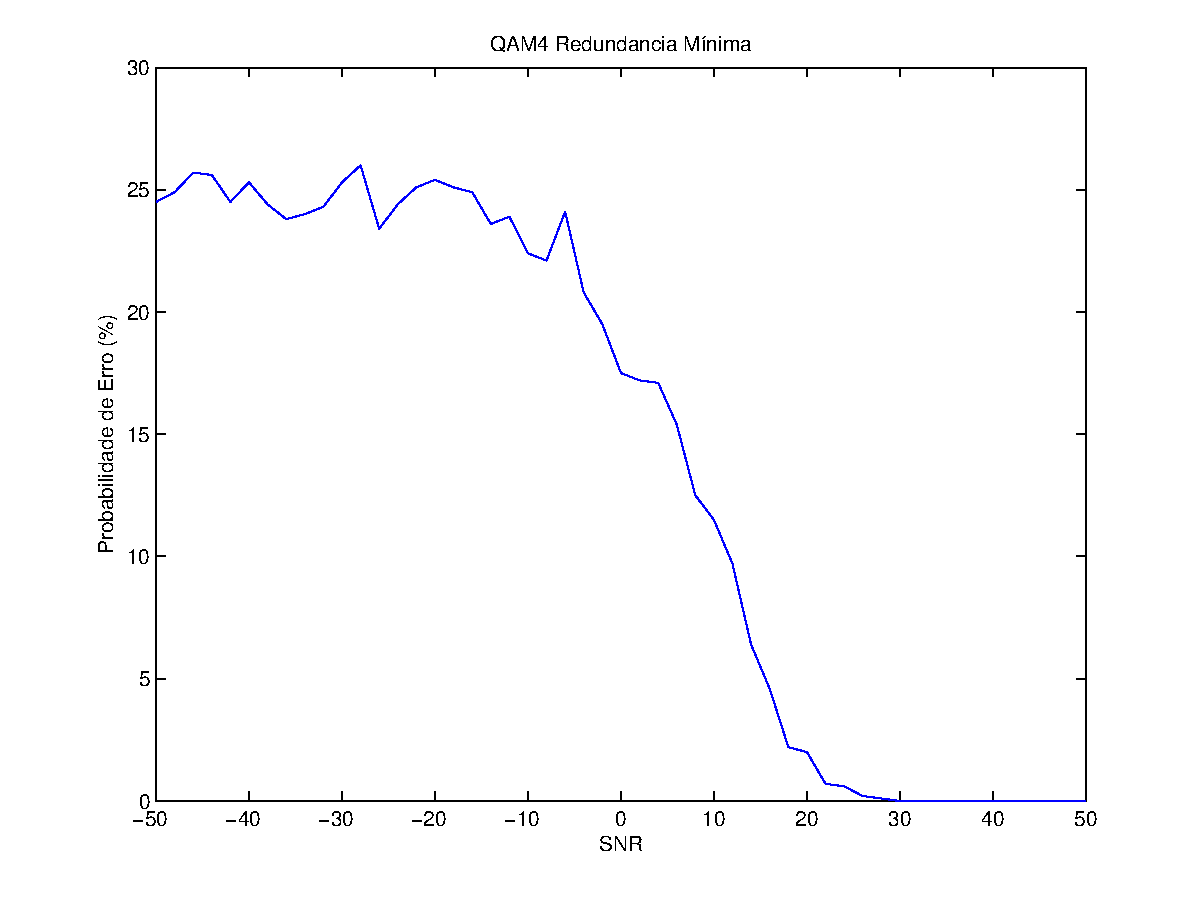
\includegraphics[width=8cm]{canalfixo/canalfixo_redunmin-QAM4-n_s-1000.pdf}
    \end{minipage}
    \caption{Erro de símbolos x SNR (Redundância Mínima canal fixo) BPSK a esquerda e QAM4 a direita}
    \label{fig:canalfixo_redunmin}
\end{figure}

\mysubsection{Overlap and Save}

\begin{figure}[H]
    \centering
    \begin{minipage}{.5\textwidth}
        \centering
        \includegraphics[width=8cm]{ovsav/ovsav-BPSK-n_s-1000-N_canais_10000.pdf}
    \end{minipage}%
    \begin{minipage}{0.5\textwidth}
        \centering
        \includegraphics[width=8cm]{ovsav/ovsav-QAM4-n_s-1000-N_canais_10000.pdf}
    \end{minipage}
    \caption{Erro de símbolos x SNR (Overlap and Save utilizando 10000 canais e sequência com 1000 símbolos) BPSK a esquerda e QAM4 a direita}
        \label{fig:ovsav-n_s-1000-N_canais_10000}
\end{figure}

\mysubsection{Overlap and Add A}

\begin{figure}[H]
    \centering
    \begin{minipage}{.5\textwidth}
        \centering
        \includegraphics[width=8cm]{ovadd_invcicl/ovadd_invcicl-BPSK-n_s-1000-N_canais_10000.pdf}
    \end{minipage}%
    \begin{minipage}{0.5\textwidth}
        \centering
        \includegraphics[width=8cm]{ovadd_invcicl/ovadd_invcicl-QAM4-n_s-1000-N_canais_10000.pdf}
    \end{minipage}
    \caption{Erro de símbolos x SNR (Overlap and Add A utilizando 10000 canais e sequência com 1000 símbolos) BPSK a esquerda e QAM4 a direita}
        \label{fig:ovadd_invcicl-n_s-1000-N_canais_10000}
\end{figure}


\mysubsection{Overlap and Add B}

\begin{figure}[H]
    \centering
    \begin{minipage}{.5\textwidth}
        \centering
        \includegraphics[width=8cm]{ovadd_ofdm/ovadd_ofdm-BPSK-n_s-1000-N_canais_10000.pdf}
    \end{minipage}%
    \begin{minipage}{0.5\textwidth}
        \centering
        \includegraphics[width=8cm]{ovadd_ofdm/ovadd_ofdm-QAM4-n_s-1000-N_canais_10000.pdf}
    \end{minipage}
    \caption{Erro de símbolos x SNR (Overlap and Add B utilizando 10000 canais e sequência com 1000 símbolos) BPSK a esquerda e QAM4 a direita}
    \label{fig:ovadd_ofdm-n_s-1000-N_canais_10000}
\end{figure}


\mysubsection{Redundância Mínima}

\begin{figure}[H]
    \centering
    \begin{minipage}{.5\textwidth}
        \centering
        \includegraphics[width=8cm]{redunmin/redunmin-BPSK-n_s-1000-N_canais_10000.pdf}
    \end{minipage}%
    \begin{minipage}{0.5\textwidth}
        \centering
        \includegraphics[width=8cm]{redunmin/redunmin-QAM4-n_s-1000-N_canais_10000.pdf}
    \end{minipage}
    \caption{Erro de símbolos x SNR (Overlap and Save utilizando 10000 canais e sequência com 1000 símbolos) BPSK a esquerda e QAM4 a direita}
    \label{fig:redunmin-n_s-1000-N_canais_10000}
\end{figure}


\mysubsection{Comparação}


Comparando todos os gráficos de canais fixos (figura \ref{fig:canalfixo_ovsav} a \ref{fig:canalfixo_redunmin}
, é possível perceber algumas semelhanças entre eles, embora possuam divesos picos. Todos encontram-se próximos de 25\% de erro com -50$dB$ e 5\% de erro próximo de 10$dB$. 
Tomando como causa da existência dos picos o fato de estar sendo usado somente um canal, ao aumentar o número de canais pode-se esperar uma suavização na curva.
Os 25\% de erro a -50$dB$ são basicamente símbolos que acabaram sendo gerados erroneamente na parte de decisão e na média acabaram sendo parecidos com os da sequência original, o que acaba sendo relativamente fácil, já que existem no máximo 4 símbolos diferentes nos casos usados (2 para o BPSK e 4 para o QAM4).
Para conhecer melhor a distribuição seria necessário utilizar sequências de diversos tamanhos e comparar as taxas de erro, com o fim de melhor esclarecer a variância entre os valores encontrados.

Aumentando o número de canais, como vemos nas figuras \ref{fig:ovsav-n_s-1000-N_canais_10000} a \ref{fig:redunmin-n_s-1000-N_canais_10000}, de fato as curvas foram suavizadas e agora assemelham-se a variações de sigmóides, mas com o mesmo perfil de 25\% de erro perto de -50$dB$ e 5\% perto de 10$dB$.
As diferenças entre eles podem ser vistas em que SNR os erros se aproximam de 1\%. Vemos que enquanto nos de redundância mínima são necessários até 40$dB$ de SNR nos outros são necessários menos de 20$dB$.
E comparando entre todos, o Overlap and Save (figura \ref{fig:ovsav-n_s-1000-N_canais_10000}) tem a melhor resposta, obtendo os menores erros de símbolos.



\mysection{Conclusão}
Com este trabalho pode-se aprender o quanto é prático a simulação de métodos de transmissão de sinais e sua análise através de programas de cálculo matricial como o \Matlab.\\ Pode-se ver também como esses diversos métodos de transmissão podem ser utilizados e com o SNR apropriado podem ser considerados altamente robustos e realizando na maior parte das vezes reconstrução perfeita do sinal transmitido quando chega-se ao receptor, obviamente quando tais métodos são amparados por ótimas estimações dos canais por onde o sinal trafega, algo que ainda é altamente difícil, já que na natureza nada é estático e fixo, mas sim altamente dinâmico. O que pode auxiliar esses tipos de problemas é a realização de uma forma de realimentação para utilizar oa estimação anterior para a fomração da estimação atual e consequente diagonalização do canal para a equalização.

\bibliographystyle{plain}
\bibliography{bibliografia}
\end{document}